
\documentclass[12pt,a4paper]{article}

% Packages
\usepackage[a4paper,margin=1in]{geometry}
\usepackage[T1]{fontenc}
\usepackage{newtxtext,newtxmath}
\usepackage{graphicx}
\usepackage{array,tabularx}
\usepackage{fancyhdr}
\usepackage{tikz}
\usepackage{xcolor}
\usepackage{float}
\usepackage{amsmath}
\usepackage[hidelinks]{hyperref}

% Paragraph formatting
\setlength{\parindent}{0pt}
\setlength{\parskip}{6pt}
\renewcommand{\arraystretch}{1.3}

% Page border
\AddToHook{shipout/background}{%
  \begin{tikzpicture}[remember picture,overlay]
    \draw[line width=1.2pt]
      ([xshift=0.45cm,yshift=-0.45cm]
      current page.north west)
      rectangle
      ([xshift=-0.45cm,yshift=0.45cm]
      current page.south east);

    \draw[line width=0.5pt]
      ([xshift=0.53cm,yshift=-0.53cm]
      current page.north west)
      rectangle
      ([xshift=-0.53cm,yshift=0.53cm]
      current page.south east);
  \end{tikzpicture}%
}

% Footer
\pagestyle{fancy}
\fancyhf{}
\fancyfoot[L]{\textbf{\thepage}\,|\,P a g e}
\renewcommand{\headrulewidth}{0pt}
\renewcommand{\footrulewidth}{0.4pt}
\usetikzlibrary{positioning}
\usepackage{graphicx}
\usepackage{float}
\begin{document}

% ---------- TITLE PAGE ----------
\begin{titlepage}
\thispagestyle{fancy}
\centering

\vspace*{0.8cm}

% University logo placeholder
{\Huge\textbf{VIT}\par}
\vspace{0.2cm}
{\large Vellore Institute of Technology\par}


\vspace{0.8cm}

{\large\textbf{SAS}\par}

\vspace{0.6cm}

{\large\textbf{Fall Semester 26-27}\par}

\vspace{1cm}

{\Large\bfseries
PHY1901: Electronic Instrumentation\par}

\vspace{0.8cm}

{\large\bfseries
Professor -- Leema Rose Viannie\par}

\vspace{1cm}

{\Large\bfseries
LiDetector\par}

\vspace{1.3cm}

\begin{tabularx}{\textwidth}{
  >{\centering\arraybackslash}X
  >{\centering\arraybackslash}X
  >{\centering\arraybackslash}X}

\textbf{Aditya Kamath} &
\textbf{Jagan P} &
\textbf{Anand Krishna P E}\\

23MPI0007 &
23MPI0008 &
23MPI0001\\[0.7cm]

\end{tabularx}

\vfill
\end{titlepage}

% ---------- TABLE OF CONTENTS ----------
\clearpage
\thispagestyle{fancy}

\vspace*{1cm}

\begin{center}
{\Large\bfseries TABLE OF CONTENTS}
\end{center}

\vspace{0.6cm}

\begin{center}
\begin{tabular}{
|>{\centering\arraybackslash}p{1.5cm}
|>{\centering\arraybackslash}p{8cm}
|>{\centering\arraybackslash}p{1.8cm}|}

\hline
\textbf{SR. NO.} &
\textbf{TITLE} &
\textbf{PAGE NO.}\\
\hline
1 & Abstract & 2\\ \hline
2 & Introduction & 2\\ \hline
3 & Problem Statement & 3\\ \hline
4 & Flowchart & 3\\ \hline
5 & Methodology & 4\\ \hline
6 & Modelling & 5-6\\ \hline
7 & Block Diagram & --\\ \hline
8 & Design & --\\ \hline
9 & Hardware Implementation & --\\ \hline
10 & Results and Outcome & --\\ \hline
11 & Conclusion & --\\ \hline
12 & References & --\\ \hline

\end{tabular}
\end{center}

\clearpage

\section*{\textbf{ABSTRACT}}
LiDetector, a humorous acronym that stands for Live audio detector, is a live spectrogram analyzer. It is designed to be lightweight and pocket-sized, which aides its use as a field-working device for ornithologists and entomologists in any terrain. A spectrogram analyser is a device that is used to analyse and visually represent an audio signal in the frequency domain over a period of time. LiDetector uses standard open source libraries to implement a FFT (Fast Fourier Transform) on captured audio signals and combines them with a standard heat map to enable collaboration among academics.

\section*{\textbf{INTRODUCTION}}
Sound is a mechanical wave that propagates through a medium and can be characterized by parameters such as frequency, amplitude, and wavelength. The analysis of sound waves plays an important role in understanding the characteristics of audio signals and studying the acoustic properties of different environments. In many applications, it is necessary to examine not only the amplitude of a sound signal but also its frequency composition and how it varies with time.

A spectrogram is a visual representation of the frequency content of a signal over time. It provides information about the distribution and intensity of different frequency components, making it useful for analysing complex sound signals. In a typical spectrogram, time is represented along the horizontal axis, frequency along the vertical axis, and signal intensity is indicated using different colours. This representation makes it possible to observe changes in the spectral characteristics of sound that may not be easily identified from a conventional waveform.

The generation of a spectrogram involves digital signal processing techniques. The Fast Fourier Transform (FFT) is commonly used to convert sampled signals from the time domain into the frequency domain. By applying this transformation to successive portions of an audio signal, the frequency components can be examined as they change over time. Frequency scaling and colour mapping are then used to present the processed information in a form that is easier to interpret.

The aim of this project is to develop a spectrogram analyser specifically for sound waves. The project explores the principles of audio signal acquisition, frequency-domain analysis, and graphical representation of spectral information. Such an analyser can be useful for studying ambient noise, examining the frequency characteristics of audio signals, and understanding the acoustic behaviour of different environments. It also provides a practical demonstration of the application of signal-processing techniques to sound analysis.
\newpage
\section*{\textbf{PROBLEM STATEMENT}}

\section*{\textbf{FLOWCHART}}

The flowchart illustrates the general sequence of
operations involved in the spectrogram analyser,
from sound acquisition to the visual representation
of its frequency components.

\begin{figure}[h!]
\centering
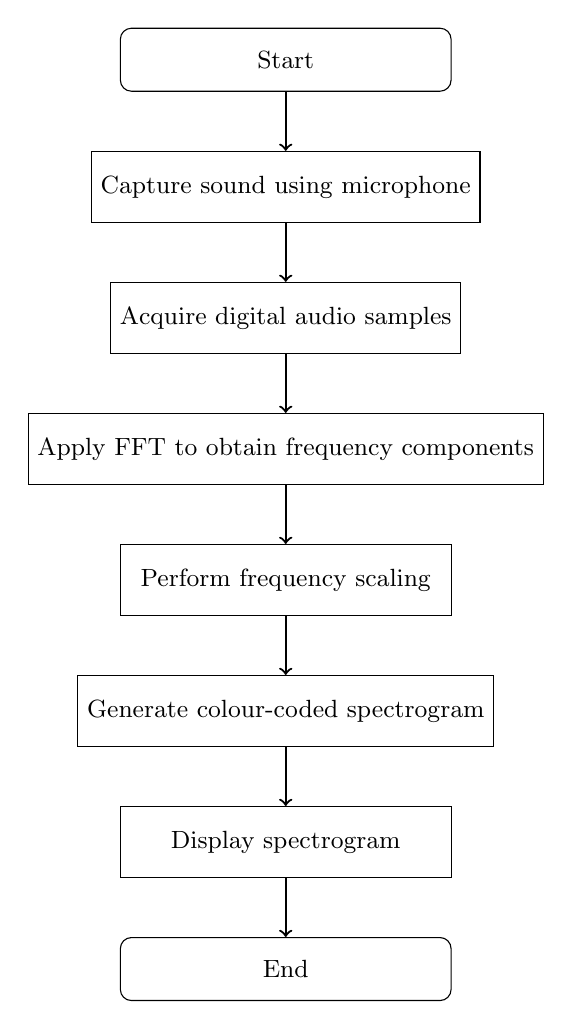
\begin{tikzpicture}[
    node distance=0.75cm,
    every node/.style={font=\small, align=center},
    startstop/.style={
        rectangle, rounded corners,
        draw, minimum width=4.2cm,
        minimum height=0.8cm
    },
    process/.style={
        rectangle, draw,
        minimum width=4.2cm,
        minimum height=0.9cm
    },
    arrow/.style={->, thick}
]

\node[startstop] (start) {Start};

\node[process, below=of start] (audio)
{Capture sound using microphone};

\node[process, below=of audio] (digitise)
{Acquire digital audio samples};

\node[process, below=of digitise] (fft)
{Apply FFT to obtain frequency components};

\node[process, below=of fft] (scale)
{Perform frequency scaling};

\node[process, below=of scale] (heatmap)
{Generate colour-coded spectrogram};

\node[process, below=of heatmap] (display)
{Display spectrogram};

\node[startstop, below=of display] (stop)
{End};

\draw[arrow] (start) -- (audio);
\draw[arrow] (audio) -- (digitise);
\draw[arrow] (digitise) -- (fft);
\draw[arrow] (fft) -- (scale);
\draw[arrow] (scale) -- (heatmap);
\draw[arrow] (heatmap) -- (display);
\draw[arrow] (display) -- (stop);

\end{tikzpicture}
\caption{Flowchart of the proposed spectrogram analyser}
\end{figure}

\newpage
\section*{\textbf{METHODOLOGY}}
The methodology of the proposed spectrogram analyser
involves the acquisition of sound signals, digital
signal processing, frequency analysis, and graphical
visualisation. The system is designed to represent
the frequency components of sound and their variation
over time.

\subsection*{1. Audio Acquisition}

A microphone is used to capture sound waves from the
surrounding environment. The sound signal is converted
into an electrical signal that represents the acoustic
variations of the input.

\subsection*{2. Digital Signal Acquisition}

The audio signal must be converted into digital samples
before it can be processed by the Raspberry Pi 3.
The digitised samples provide the input data required
for subsequent signal-processing operations. The
specific audio-input interface depends on the
microphone and its connection to the system.

\subsection*{3. Fast Fourier Transform (FFT)}

The acquired digital audio samples are analysed using
the Fast Fourier Transform (FFT). This technique
converts a finite sequence of samples from the time
domain into a frequency-domain representation,
allowing the frequency components present in the
sound signal to be examined.

\subsection*{4. Frequency Scaling}

The frequency components obtained from the FFT are
mapped onto an appropriate frequency scale. This
helps represent the spectral information clearly and
makes it easier to examine the distribution of
frequencies in the input sound.

\subsection*{5. Heat-Map Generation}

The processed frequency information is represented
using a colour-coded heat map. Different colours
indicate different signal magnitudes, allowing
variations in spectral intensity to be observed
visually over time.

\subsection*{6. Spectrogram Display}

The generated spectrogram is prepared for visual
presentation. The Raspberry Pi 3 forms the main
processing platform, while the 3.5-inch TFT LCD is
included as part of the hardware setup. The final
display configuration will depend on the software
and display interface used in the implementation.
\newpage
\section*{\textbf{MODELLING}}
The proposed spectrogram analyser consists of hardware
components that support audio processing and visualisation.
The Raspberry Pi 3 acts as the main processing unit, while
the microphone captures sound from the surrounding
environment. The IQaudio DAC Pro and the TFT LCD form part
of the hardware setup. The major components used in the
project are described below.
\subsection*{1. Raspberry Pi 3}

The Raspberry Pi 3 is the main processing unit of the
proposed system. It executes the software required for
signal processing and spectrogram generation. The audio
samples are processed using techniques such as the Fast
Fourier Transform (FFT), after which the frequency
information is represented visually.

\begin{figure}[H]
    \centering
    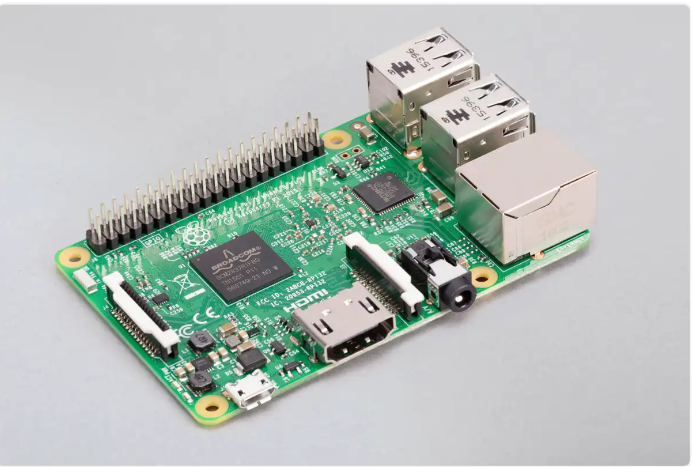
\includegraphics[width=0.45\textwidth]
    {Rasberry PI.png}
    \caption{Raspberry Pi 3 used in the project.}
    \label{fig:raspberry-pi3}
\end{figure}
\subsection*{2. IQaudio DAC Pro}

The IQaudio DAC Pro is a digital-to-analogue converter
designed for the Raspberry Pi. It is included in the
hardware setup as an audio output component. Its role
in the complete system depends on the audio input and
output connections used in the implementation.

\begin{figure}[H]
    \centering
    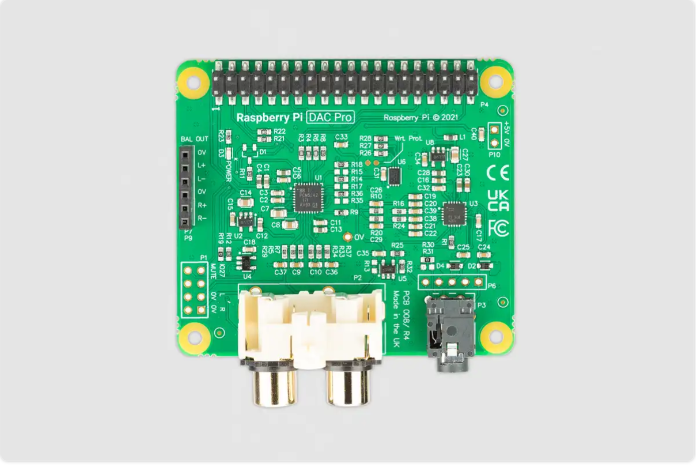
\includegraphics[width=0.45\textwidth]
    {IQaudio DAC Pro.jpg}
    \caption{IQaudio DAC Pro audio interface.}
    \label{fig:iqaudio-dac}
\end{figure}

\subsection*{3. Microphone}

The microphone captures sound waves from the surrounding
environment and converts them into an electrical audio
signal. This signal must be acquired as digital samples
before it can be processed by the Raspberry Pi. The
method of acquisition depends on the type of microphone
and the interface used to connect it to the system.

\begin{figure}[H]
    \centering
    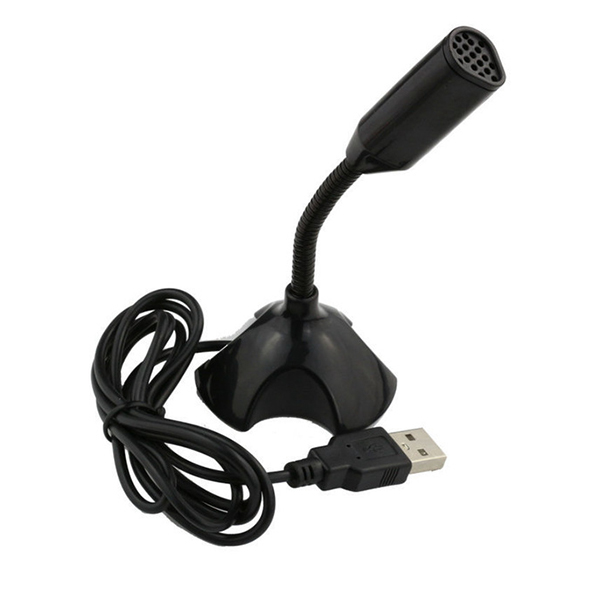
\includegraphics[width=0.35\textwidth]
    {Microphone.jpg}
    \caption{Microphone used to capture sound signals.}
    \label{fig:microphone}
\end{figure}

\subsection*{4. 3.5-inch LCD Display (ILI9486)}

The 3.5-inch LCD display is included to present
the generated spectrogram visually. The processed
frequency information can be represented using a
colour-coded display, allowing variations in the
spectral content of the sound signal to be observed.


\begin{figure}[H]
    \centering
    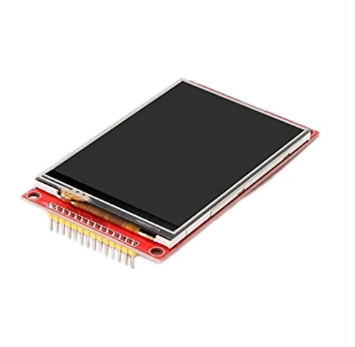
\includegraphics[width=0.45\textwidth]
    {LCD Screen.png}
    \caption{3.5-inch LCD display used in the project.}
    \label{fig:tft-display}
\end{figure}

\newpage
\section*{\textbf{BLOCK DIAGRAM}}
A basic Block Diagram is used to describe the implementation of LiDetector
\section*{\textbf{DESIGN}}
The device can be used in two main modes, both of which must be supported by the design of the device. The two main modes are 'Handheld' and 'Headless'. The Handheld mode is used by field researchers to visit the sighting and research locations to collect environmental sound samples. This mode allows for greater flexibility while focusing on a specific wildlife entity say, a tagged bird or an insect population. The Headless mode is used to collect data from a fixed site to collect varied data about a certain ecosystem and to scour areas for the presence of wildlife entities.

The Handheld mode comes attached with the TFT screen for easy access to the live spectrogram. It can be easily converted into headless mode by simply detaching the TFT screen and connecting a mobile device or a computer to monitor the frequencies from a remote location. 

\section*{\textbf{HARDWARE IMPLEMENTATION}}
[Basic Pictures and a little bit of text describing the setup]

\section*{\textbf{RESULTS AND OUTCOME}}

[Pictures and a little bit of text]

\section*{\textbf{CONCLUSION}}
LiDetector provides a practical approach to analysing sound waves through a live spectrogram. By capturing audio signals, applying the Fast Fourier Transform (FFT), and displaying the frequency components using a colour-coded heat map, the device makes it easier to observe changes in sound over time. Its handheld and headless modes are intended to provide flexibility for field researchers, including ornithologists and entomologists, who may need to monitor wildlife sounds in different environments. The proposed system also demonstrates how digital signal-processing techniques can be applied using a compact, Raspberry Pi-based platform. Further work can focus on completing the hardware implementation, testing the analyser with known audio signals, and evaluating its performance in field conditions.

\section*{\textbf{REFERENCES}}

[References will be added here.]
\end{document}
